% !TEX root = ../seapp-manual.tex

% Chapter 3 - Set up and run a new SEA++ scenario

\chapter{Set up and run a new SEA++ scenario}
\label{ch:run-scenario}

SEA++ is distributed with a complete set of examples that are ready to use. However, the process to build a new SEA++ scenario is substantially identical to that of INET.

In the following example is shown how to set up a new simple scenario in which there are a client and a server.

\paragraph{\nth{1} step - make the folder}
As in INET, the \nth{1} step is to make the folder that will contain all the new files, e.g. scenario.
%
\begin{lstlisting}[language={terminal}]
@~/seapp-0.99/inet/examples/@ mkdir scenario
@~/seapp-0.99/inet/examples/@ cd scenario
\end{lstlisting}


\paragraph{\nth{2} step - network description}
As in INET, the \nth{2} step is to edit the \texttt{.ned} file that contains the network description, e.g. \texttt{scenario.ned}.
%
\begin{lstlisting}[language={ned}, caption={scenario.ned}, label={lst:build-scenario-ned}]
package inet.examples.inet.scenario;

import inet.networklayer.autorouting.ipv4.IPv4NetworkConfigurator;
import inet.nodes.inet.StandardHost;
import inet.globalfilter.GlobalFilter;

network scenario
{
  parameters:
    string attackConfigurationFile = default("none");
    double n;

  submodules:
    globalFilter: GlobalFilter;
    client: StandardHost;
    server: StandardHost;
    configurator: IPv4NetworkConfigurator;
        
  connections allowunconnected:
    client.pppg++ <--> { datarate = 10Mbps; } <--> server.pppg++;
    globalFilter.nodes++ <--> client.global_filter;
    globalFilter.nodes++ <--> server.global_filter;
    
}
\end{lstlisting}

In this step, is fundamental to:
%
\begin{itemize}
\item add the the string parameter \texttt{attackConfigurationFile} to the network;
\item import the GlobalFilter class, declare a GlobalFilter submodule and connect it to all the other nodes.
\end{itemize}

\paragraph{\nth{3} step - edit omnetpp.ini}
As in INET, the \nth{3} step is to edit the \texttt{omnetpp.ini} file. In this step is fundamental to bind the configuration(s) with the ACF(s), by overwriting the name of the network parameter \texttt{attackConfigurationFile} with the name of a particular ACF.
%
\begin{lstlisting}[language={ini}]
[General]
network = scenario
@sim-time-limit@  = 600s

// General settings ...

// Config(s) specific settings
[Config attack-example]
**.attackConfigurationFile = attack-example.xml

[Config attack-example2]
**.attackConfigurationFile = attack-example2.xml

// ...
\end{lstlisting}

\paragraph{\nth{4} step - add the ACF}
The \nth{4} and last step is to add the ACF(s) in the folder.

\paragraph{Run the simulation}
The simulation is ready to run. In the terminal, call \texttt{run\_inet} that is in the \texttt{src} folder:
%
\begin{lstlisting}[language={terminal}]
@~/seapp-0.99/inet/examples/scenario@ ../../src/run_inet $*
\end{lstlisting}
%
It will start the simulation supported by the GUI, as shown in figure~\ref{img:appendix-scenario}. Be carefull to specify well the path from the current folder (i.e. the simulation folder) to the \texttt{src} folder. 

To run the simulation in express mode without use the GUI, type:
\begin{lstlisting}[language={terminal}]
@~/seapp-0.99/inet/examples/scenario@ ../../src/run_inet -u Cmdenv -f omnetpp.ini
\end{lstlisting}
%
\begin{landscape}
\begin{figure}[b]
\centering
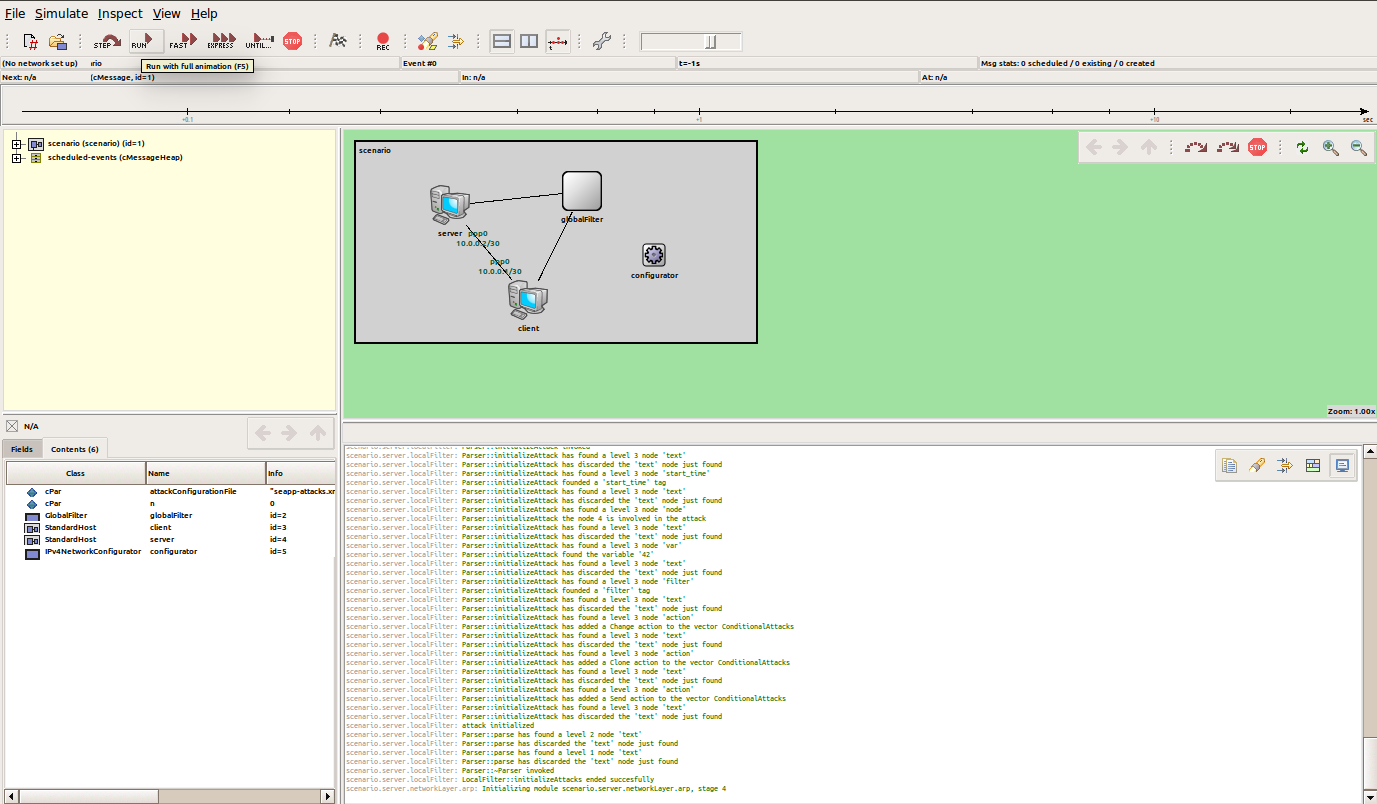
\includegraphics[width=.9\columnwidth]{appendix-scenario}
\caption{Simulation scenario}
\label{img:appendix-scenario}
\end{figure}
\end{landscape}









